% EF5342 Week 6 — Market Efficiency
% Beamer conversion from week6_MarketEfficiency.pptx (64 source slides -> 44 frames).
% Compile: pdflatex week6_MarketEfficiency.tex
% Each frame carries a [src: ...] comment mapping back to source slides.
\documentclass[aspectratio=169]{beamer}
\usepackage{../ef5342}

\title{EF5342 Financial Systems, Markets and Instruments}
\subtitle{Week 6 --- Market Efficiency}
\author{Prof.\ Weikai Li}
\institute{City University of Hong Kong}
\date{Semester B 2026--2027}

\begin{document}

% ============ INTRODUCTION ============

% [src: 1]
\begin{frame}
\titlepage
% Title-page background image (slide01_img.jpg) dropped — decorative.
\end{frame}

% [src: 2, 3]
\begin{frame}{Market Efficiency: The Most Important Debate in Finance}
Why does this debate matter more than any other in finance? Because the answer determines whether prices do their job --- guiding the allocation of capital --- and whether anyone can consistently beat the market.
\vspace{0.6em}
\textbf{Agenda}
\begin{itemize}
  \item Efficient Markets Hypothesis
  \item Evidence for and against market efficiency
  \item Anomalies: facts and explanations
  \item Smart Beta ETFs
\end{itemize}
\end{frame}

% [src: 4]
\begin{frame}{Efficient Markets Hypothesis (EMH)}
\begin{description}
  \item[Efficient market] Prices of securities \textbf{fully reflect all available information}
\end{description}
\vspace{0.3em}
Competition among investors ensures that new information gets incorporated into prices right away. Since new information is unpredictable and random by definition, so are price changes:
\begin{itemize}
  \item Price changes should follow a \textbf{random walk}
\end{itemize}
\vspace{0.3em}
\begin{columns}
\begin{column}{0.52\textwidth}
\begin{figure}
\centering

\includegraphics[height=0.50\textheight,keepaspectratio]{figures/slide04_img.png}
\end{figure}
\end{column}
\begin{column}{0.44\textwidth}
\small Real stock prices look much like a simulated random walk --- hard to tell them apart.
\end{column}
\end{columns}
\note{Price changes should be random and unpredictable. Implication: price always reflects all current knowledge and all available information.}
\end{frame}

% [src: 5, 6]
\begin{frame}{News Response and Market Efficiency}
\textbf{Timely responses imply efficient markets:} cumulative abnormal return (CAR) \emph{jumps} on the announcement day for good news (up) and bad news (down), with \textbf{no further drift} afterwards. Key feature of efficient markets: \emph{no predictability}.
\vspace{0.5em}

\textbf{Untimely responses imply inefficiency:}
\begin{description}
  \item[Leakage] Prices react \emph{too soon} --- they drift up before the news announcement, as insiders learn the information
  \item[Drift] Prices react \emph{with a delay} --- they keep drifting in the news direction \emph{after} the announcement
\end{description}
\note{This figure shows the response of stock prices to new info in a perfectly efficient market. CAR = cumulative abnormal return: see the jump at the announcement date and no further drift afterwards. Prices reflect the new info including the likely magnitude of the premium/discount by the end of the announcement day. Studies show rapid response to corporate dividend or earnings announcements.}
\end{frame}

% [src: 7]
\begin{frame}{Stock Price Reaction to Takeover Announcement}
\begin{figure}
\centering
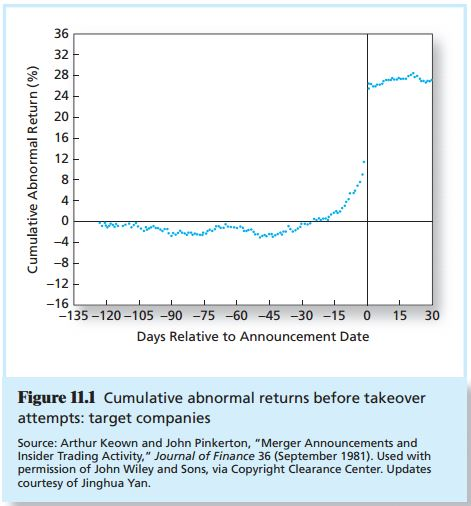
\includegraphics[height=0.62\textheight,keepaspectratio]{figures/slide07_img.jpg}
\end{figure}
\vspace{0.3em}
\textbf{Question:} why do prices trend \emph{up} before the takeover announcement?
\note{Looks pretty efficient. If you are an ordinary investor, difficult to profit from this type of information.}
\end{frame}

% [src: 8, 9]
\begin{frame}{Case: EntreMed (Huberman \& Regev 2001)}
\begin{columns}
\begin{column}{0.46\textwidth}
\small
\begin{itemize}
  \item \textbf{27 Nov 1997:} \emph{Nature} reports a cancer-research breakthrough, mentioning ENMD as owning licensing rights
  \item \textbf{3 May 1998:} Sunday \emph{New York Times} reports the same story on the front page of the business section
  \item \textbf{12 Nov 1998:} \emph{Wall Street Journal} reports that the results in the 3 May Times article cannot be independently replicated
\end{itemize}
\end{column}
\begin{column}{0.50\textwidth}
\begin{figure}
\centering
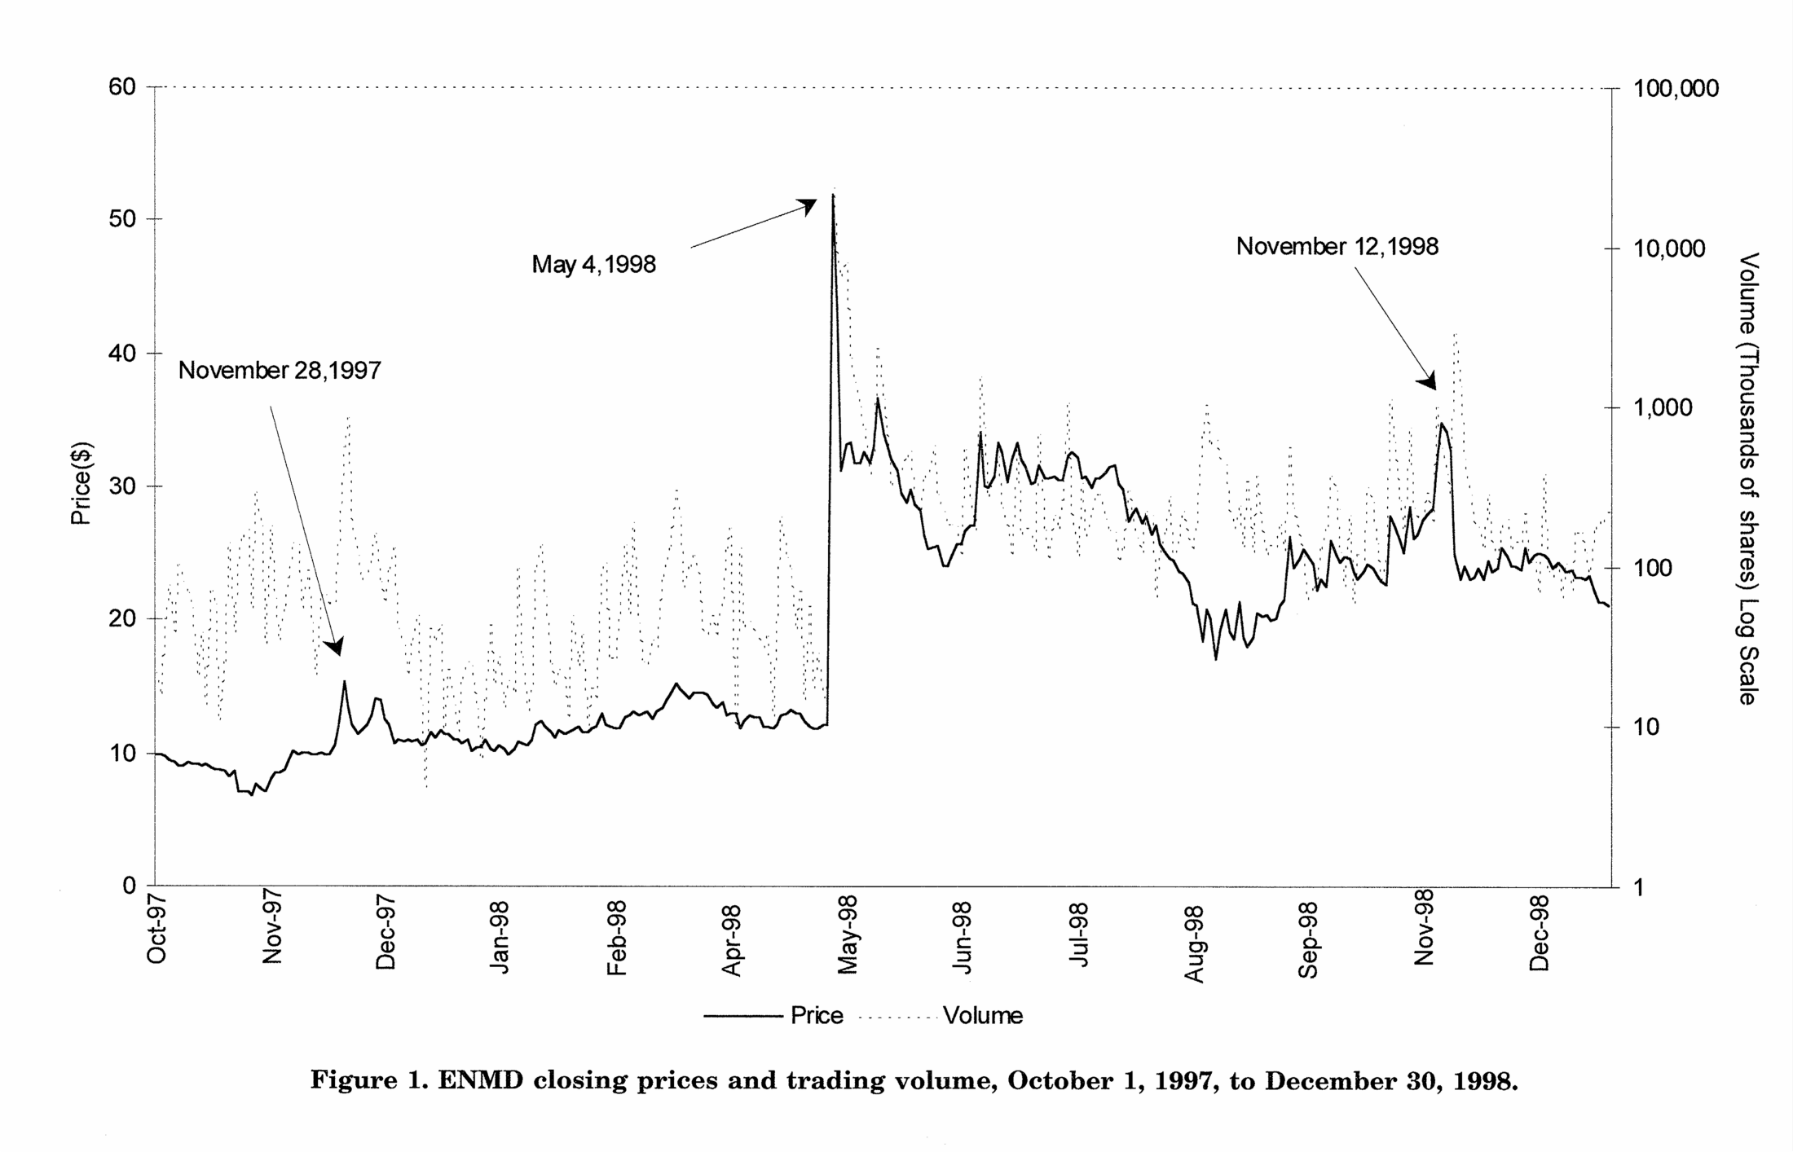
\includegraphics[height=0.56\textheight,keepaspectratio]{figures/slide09_img_flat.png}
\end{figure}
\end{column}
\end{columns}
\note{EntreMed is a small biotech company with rights to commercialize a potentially cancer-curing process. The 27 Nov article also appeared in the New York Times on page A28; CNN and CNBC also mentioned the story. On 11/28, ENMD itself issued a press release covering the news and the company's licensing rights. What explains the price movement of EntreMed on Monday 4 May 1998 shown in this picture? EntreMed's price rose from 12.063 at the Friday close to open at 85 and closed near 52 on Monday. It closed above 30 in the 3 following weeks. The enthusiasm spilled over to other biotech stocks.}
\end{frame}

% [src: 10]
\begin{frame}{Why Do We Care About Market Efficiency?}
Deviations from efficiency may offer profitable opportunities to better-informed traders --- \emph{at the expense of less-informed traders}.
\vspace{0.4em}

Inefficient markets $\Rightarrow$ mispriced securities $\Rightarrow$ suboptimal resource allocation:
\begin{itemize}
  \item \textbf{Overvalued} firms can raise capital too cheaply and \textbf{overinvest}
  \item \textbf{Undervalued} firms may pass up profitable opportunities because their cost of capital is too high
\end{itemize}
\vspace{0.4em}
Thus, \textbf{efficient security prices help allocate resources efficiently}.
\end{frame}

% ============ EMH: THREE FORMS ============

% [src: 11, 12]
\begin{frame}{Weak-Form Market Efficiency}
Market efficiency is a matter of \textbf{degree} --- it depends on how we define ``available information.'' Three increasing degrees: weak, semi-strong, strong.
\vspace{0.3em}
\begin{description}
  \item[Weak form] Stock prices already reflect all information contained in the \textbf{history of past prices and trading volumes}
\end{description}
\emph{Reasoning:} if such data ever conveyed reliable signals, investors would have learned to trade on them, impounding them into prices and removing further profit opportunities --- a buy signal results in an immediate price increase.
\vspace{0.3em}

\textbf{Technical analysis} uses historical prices and volume to predict future price changes. Weak-form efficiency $\Rightarrow$ \emph{technical analysis should not work}.
\begin{center}
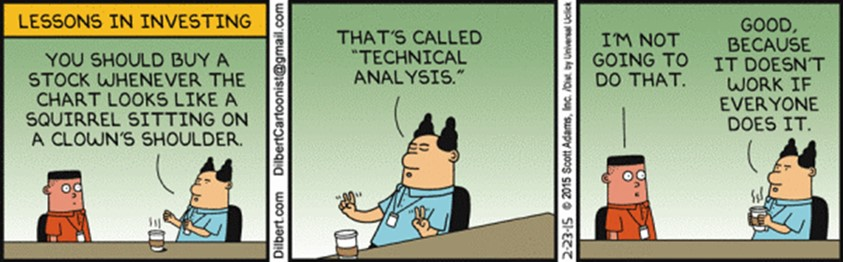
\includegraphics[height=0.22\textheight,keepaspectratio]{figures/slide12_img.png}
\end{center}
\end{frame}

% [src: 13, 14]
\begin{frame}{Semi-Strong Form Market Efficiency}
\begin{description}
  \item[Semi-strong form] Prices reflect all \textbf{publicly available information}: historical price/volume plus public information on firm fundamentals --- revenues and costs, balance-sheet strength, patents held, quality of management, etc.
\end{description}
\emph{Reasoning:} if useful, investors have learned to trade on this information, already impounding it into prices and removing further profit opportunities.
\vspace{0.3em}

\textbf{Fundamental analysis} tries to identify mispriced securities by examining economic/financial factors. Semi-strong efficiency $\Rightarrow$ \emph{fundamental analysis should not work}.
\note{Market efficiency in real time: the figure shows the reaction of stock prices to on-air stock reports during the Morning Call and Midday Call segments on CNBC. The chart plots cumulative returns beginning 15 minutes before the stock report, partitioned into positive and negative reports.}
\begin{figure}
\centering

\includegraphics[height=0.38\textheight,keepaspectratio]{figures/slide14_img.png}
\end{figure}
\end{frame}

% [src: 15]
\begin{frame}{Strong-Form Market Efficiency}
\begin{description}
  \item[Strong form] Prices reflect \textbf{all relevant information}: historical and public information \emph{plus insider information} (e.g., upcoming M\&A and earnings news)
\end{description}
\emph{Reasoning:} insiders (or their allies) have already traded on this information, impounding it into prices and removing further profit opportunities.
\vspace{0.3em}
Strong-form efficiency $\Rightarrow$ \emph{trading on insider information is also fruitless}.
\note{This version of the hypothesis is quite extreme. Indeed, much of the SEC's activity is directed toward preventing insiders from profiting by exploiting their privileged situation. They set rules that limit trading by corporate officers, directors, and substantial owners, requiring them to report trades to the SEC.}
\end{frame}

% [src: 16, 17]
\begin{frame}{Insider Trading --- and the Congress}
In financial markets, trading on insider information is highly profitable --- and insiders may not just be corporate managers.
\begin{itemize}
  \item Ziobrowski et al.\ (2004) document abnormal profits earned from mimicking the trades of U.S.\ senators
  \item Retail products now track congressional trading: the \textbf{Unusual Whales Subversive Democratic Trading ETF} (ticker NANC, Cboe BZX; $\approx$\$278M AUM, 0.72\% expense ratio as of Aug 2026)
\end{itemize}
\begin{columns}
\begin{column}{0.44\textwidth}
\begin{figure}
\centering

\includegraphics[height=0.42\textheight,keepaspectratio]{figures/slide16_img_flat.png}
\end{figure}
\end{column}
\begin{column}{0.54\textwidth}
\begin{figure}
\centering
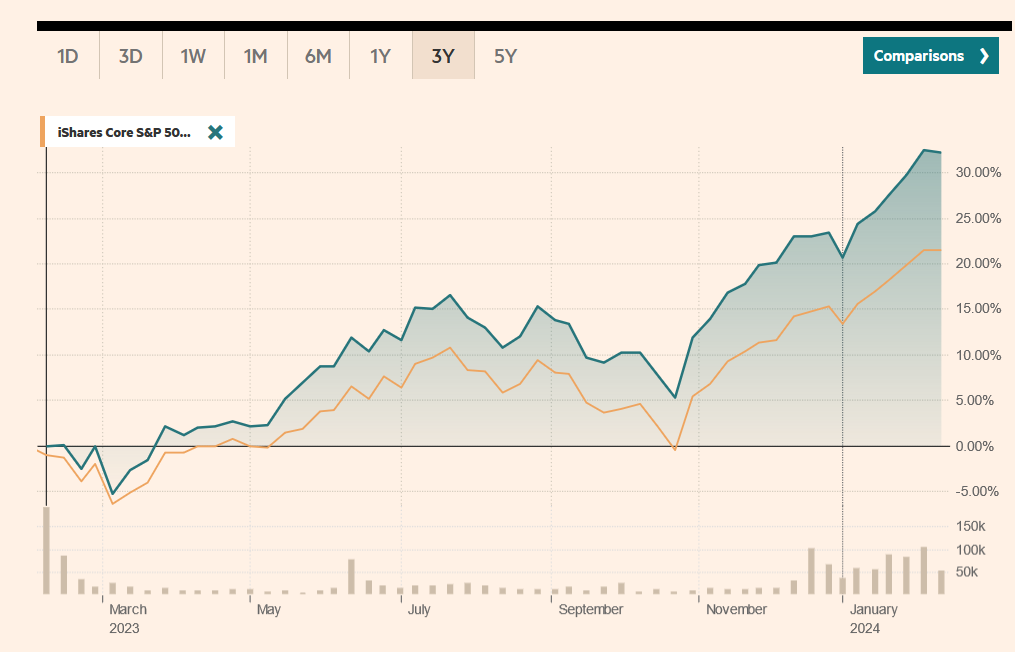
\includegraphics[height=0.42\textheight,keepaspectratio]{figures/slide16_img1_flat.png}
\end{figure}
\end{column}
\end{columns}
\note{NANC ETF (Unusual Whales Subversive Democratic Trading ETF, Cboe BZX, inception Feb 2023, 0.72\% expense ratio): \url{https://unusualwhales.com/etf/NANC}; congressional trading data: \url{https://www.quiverquant.com/} (both as of Aug 2026)}
\end{frame}

% [src: 18]
\begin{frame}{Three Forms of Market Efficiency: Summary}
\begin{table}
\centering
\small
\begin{tabular}{llll}
\toprule
\textbf{Form} & \textbf{Information reflected} & \textbf{Implication} & \\
\midrule
Weak form & Historical price/volume & Technical analysis fruitless & \\
Semi-strong & $+$ all public information & Fundamental analysis fruitless & \\
Strong form & $+$ insider information & Insider trading fruitless & \\
\bottomrule
\end{tabular}
\end{table}
\vspace{0.3em}
Each form nests the previous one --- the information set only grows.
\end{frame}

% ============ EVIDENCE ============

% [src: 19]
\section{Evidence For and Against Market Efficiency}

% [src: 20]
\begin{frame}{Evidence Against Market Efficiency}
It is not surprising that the market is not strong-form efficient:
\begin{itemize}
  \item The ability of insiders to trade profitably is well documented by academic studies
  \item The SEC closely monitors and prosecutes insider trading cases
\end{itemize}
\vspace{0.3em}
In a well-functioning market, we should at least expect \textbf{semi-strong-form} efficiency. Yet recent studies document evidence that the stock market is not even weak-form efficient: both historical prices/volume \emph{and} current firm fundamentals can predict future stock movements.
\note{We expect semi-strong because information about firms' fundamentals is widely available.}
\end{frame}

% [src: 21]
\begin{frame}{Violation of Weak-Form Efficiency: Momentum}
\textbf{Jegadeesh \& Titman (1993):} stocks with good (bad) past 6- to 12-month returns continue to do well (poorly) in the future.
\vspace{0.4em}

\textbf{Why is this a violation of weak-form efficiency?} The strategy uses \emph{only} past returns --- information already contained in prices --- yet earns abnormal profits.
\vspace{0.6em}

\begin{center}
\small Source: my calculation based on Kenneth French's data.
\end{center}
% TODO: recreate chart (native PowerPoint chart on source slide 21 — no image recovered).
\note{Why is this a violation of weak-form efficiency?}
\end{frame}

% [src: 22]
\begin{frame}{Violation of Semi-Strong Form Efficiency: Post-Earnings Announcement Drift}
Firms announcing unexpectedly \textbf{good} (bad) earnings continue to do well (poorly) over the next quarter.
\begin{itemize}
  \item The market appears to adjust to the earnings surprise only \emph{gradually}, resulting in a sustained period of price drift
\end{itemize}
\begin{figure}
\centering

\includegraphics[height=0.50\textheight,keepaspectratio]{figures/slide22_img.png}
\end{figure}
\end{frame}

% [src: 23]
\begin{frame}{Asset Bubbles}
\textbf{Asset bubbles}: for a significant period, an asset trades at a price substantially higher than its fair value --- the most dramatic form of market inefficiency and investor irrationality.
\vspace{0.4em}

\small Historical episodes, indexed to 1 at start: Tulip Mania (1634--1637, green; peaks around 50--60x); Japanese stocks (1982--1992, light blue; $\sim$80x at peak); Tech/Dot-com (1994--2002, cyan; $\sim$20--30x); Mississippi Bubble (1718--1720, blue; 20--30x); South Sea Bubble (1719--1721, purple).
\begin{figure}
\centering
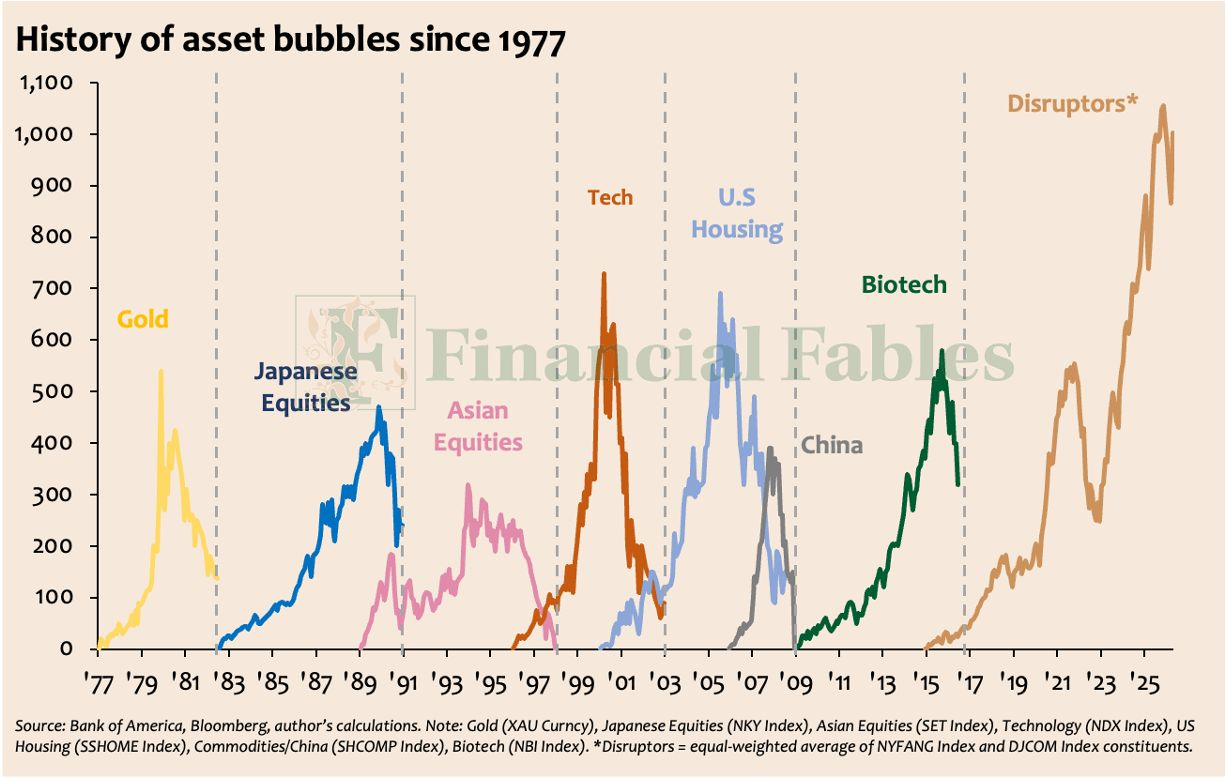
\includegraphics[height=0.50\textheight,keepaspectratio]{figures/slide23_img.jpg}
\end{figure}
\end{frame}

% [src: 24]
\begin{frame}{The Dot-Com Bubble in One Chart}
\begin{columns}
\begin{column}{0.52\textwidth}
\begin{itemize}
  \item NASDAQ rose $\sim$400--600\% from 1995 to the peak (1,000 $\to$ 5,000+)
  \item Fell $\sim$78\% from peak to trough (2000--2002)
  \item Many dot-com companies went to zero; even survivors like Cisco took $\sim$15 years to recover their 2000 highs
\end{itemize}
\end{column}
\begin{column}{0.44\textwidth}
\begin{figure}
\centering
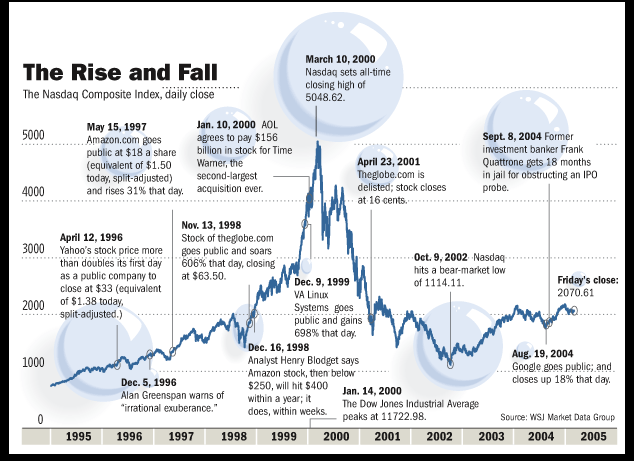
\includegraphics[width=\linewidth,keepaspectratio]{figures/slide24_img_conv.png}
\end{figure}
\end{column}
\end{columns}
\end{frame}

% [src: 25]
\begin{frame}{Mini Case: The Dot-Com Bubble (1995--2000) --- Irrational Exuberance or Rational Revolution?}
\textbf{Catalyst.} Commercialization of the World Wide Web (early 1990s) promised to reshape commerce; firms were valued on ``eyeballs'' (web traffic), user growth, and platform potential rather than earnings, cash flows, or assets.
\vspace{0.4em}

\textbf{EMH viewpoint:} the market rationally priced the \emph{option value} of dominance in a winner-take-most digital economy; high uncertainty justified high valuations.
\vspace{0.4em}

\emph{Discussion:} in 1998, was it rational to value Amazon (never profitable) above established retailers like Barnes \& Noble? Why or why not?
\end{frame}

% [src: 26]
\begin{frame}{The Bubble Inflation Mechanism (1998--2000)}
\begin{itemize}
  \item \textbf{Venture capital fuel:} easy money into startups with ``.com'' in the name
  \item \textbf{IPO frenzy:} minimal-revenue firms went public with first-day pops of 100\%+ (VA Linux: +698\% on debut)
  \item \textbf{Retail mania:} online brokerages (E*Trade) and day trading became mainstream
  \item \textbf{Media and analyst hype:} valuation metrics dismissed as ``old economy'' thinking; ``this time is different''
  \item \textbf{Momentum investing:} rising prices attracted buyers, decoupling prices from any plausible fundamentals
\end{itemize}
\end{frame}

% [src: 27]
\begin{frame}{The Prick and Collapse (2000--2002)}
\textbf{10 March 2000:} NASDAQ peaks at 5,048.62 (up from $\sim$750 in 1995). Catalysts: Fed \textbf{interest-rate hikes}; \textbf{profit warnings} from internet infrastructure firms (e.g., Cisco); \textbf{lock-up expirations} letting insiders finally sell; growing \textbf{skepticism} (Barron's ``Burning Up,'' March 2000, on cash burn rates).
\vspace{0.4em}
\textbf{Aftermath:} NASDAQ fell $\sim$78\% by October 2002; most dot-coms failed; survivors (Amazon, eBay) saw 90\%+ drawdowns; $\sim$\$5 trillion in market value evaporated.
\end{frame}

% [src: 28]
\begin{frame}{A Failure of Market Efficiency?}
\textbf{Yes:} investor irrationality (overconfidence, herd behavior, extrapolation bias); agency problems (analysts at investment banks faced underwriting conflicts and issued overly optimistic reports); asymmetric information (VCs and founders understood the fragility but had incentives to promote the narrative). ``Irrational exuberance'' --- Alan Greenspan (1996), years before the peak.
\vspace{0.4em}

\textbf{But} consider the counterargument:
\emph{``The Dot-Com Bubble proves markets are inefficient because prices clearly deviated from intrinsic value. However, it also proved efficient in the long run by rapidly allocating massive capital to a transformative technology, allowing the optimal business models to emerge through a Darwinian process. Which perspective is more compelling, and what does that tell us about the time horizon of market efficiency?''}
\end{frame}

% [src: 29, 30]
\begin{frame}{Market Efficiency and Money Making: Mutual Funds}
Another test of semi-strong efficiency: the performance of mutual fund managers, most of whose profits would come from exploiting market inefficiency.
\begin{itemize}
  \item If the market is not semi-strong efficient and managers have skill, they should \emph{consistently} outperform the index benchmark
  \item Efficient markets: no one can earn abnormal profits \emph{consistently}
\end{itemize}
\begin{figure}
\centering
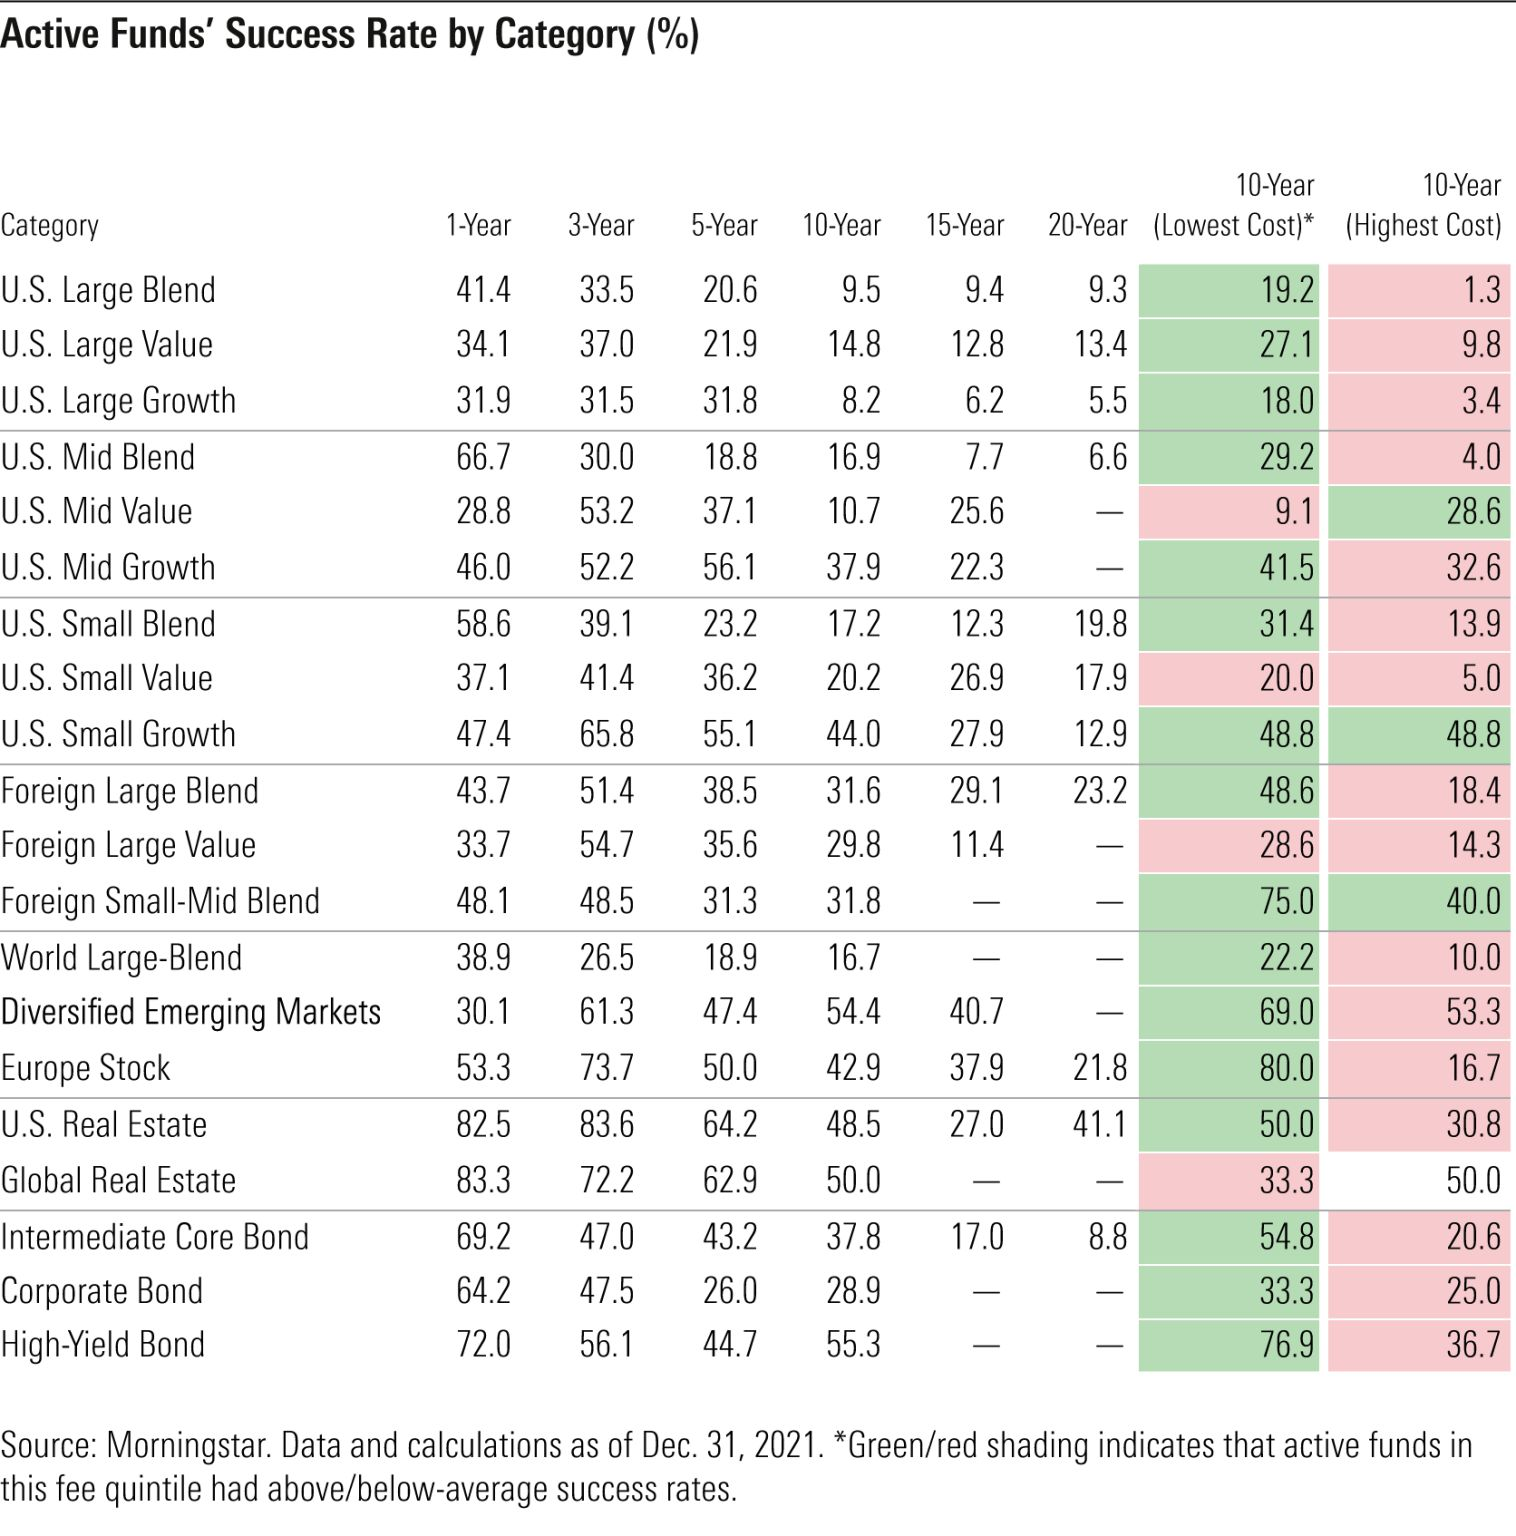
\includegraphics[height=0.42\textheight,keepaspectratio]{figures/slide30_img_conv.png}
\end{figure}
\begin{center}
\small Outperforming becomes harder the longer the evaluation window. Success rate: fraction of active funds across the 20 Morningstar categories that survived and outperformed their average passive peer.
\end{center}
\note{It is possible to find some funds outperforming in a single year; this could be luck. The EMH only states that no one can outperform consistently over time.}
\end{frame}

% ============ ANOMALIES ============

% [src: 31]
\section{Anomalies: Facts and Explanations}

% [src: 32]
\begin{frame}{Anomalies}
Patterns in stock prices that cannot be easily explained by the EMH are called \textbf{anomalies}. Practitioners are very interested --- anomalies are potential money-making machines. Recent decades have produced hundreds of documented anomalies. The most robust:
\begin{columns}
\begin{column}{0.42\textwidth}
\begin{itemize}
  \item Size effect
  \item Value premium
  \item Long-term reversal
  \item Low volatility anomaly
\end{itemize}
\end{column}
\begin{column}{0.42\textwidth}
\begin{itemize}
  \item Profitability / quality
  \item Investment
  \item Share issuance
\end{itemize}
\end{column}
\end{columns}
\end{frame}

% [src: 33]
\begin{frame}{Size Effect}
Sort stocks into 10 portfolios by \textbf{market capitalization}: small firms (decile 1) earn higher average returns than large firms (decile 10).
\vspace{0.6em}

\begin{center}
\small Source: my calculation based on Ken French's data.
\end{center}
% TODO: recreate chart (native PowerPoint chart on source slide 33 — no image recovered).
\end{frame}

% [src: 34, 35]
\begin{frame}{Value Premium --- and Competing Explanations}
Sort all stocks into 10 portfolios by \textbf{book-to-market}: value stocks (decile 10) outperform growth stocks (decile 1) on average. \small(Source: my calculation based on Ken French's data.)\normalsize
% TODO: recreate chart (native PowerPoint chart on source slide 34 — no image recovered).
\vspace{0.4em}

Why does the premium exist?
\begin{description}
  \item[Risk-based view] Value firms have higher leverage, more irreversible capital, and greater exposure to financial-distress risk in downturns --- they are inherently riskier
  \item[Behavioral view] Lakonishok, Shleifer, and Vishny (1994): investors extrapolate past growth too far, overpricing glamour stocks and underpricing value stocks
\end{description}
\vspace{0.3em}
Both explanations find some support in the data.
\end{frame}

% [src: 36, 37]
\begin{frame}{Long-Term Reversal}
Stock prices exhibit \textbf{long-term reversal}. De Bondt and Thaler (1985) --- one of the first anomaly papers --- show that stocks that performed poorly over the last 3 years tend to do very well in the following 5 years.
\begin{columns}
\begin{column}{0.50\textwidth}
\begin{figure}
\centering

\includegraphics[height=0.58\textheight,keepaspectratio]{figures/slide36_img.jpg}
\end{figure}
\end{column}
\begin{column}{0.46\textwidth}
\small Source: De Bondt and Thaler (1985)
\vspace{0.5em}

\textbf{Explanation:} investors \emph{overreact} to past firm performance --- overly pessimistic about firms with poor past performance, leading to undervaluation. Eventually they realize these loser stocks are not so bad, and prices revert in the long run.
\end{column}
\end{columns}
\end{frame}

% [src: 38, 39]
\begin{frame}{Low Volatility Anomaly}
The first principle of finance (and life) is that high risk comes with high return --- yet this principle is \emph{often violated in the market} (Baker, Bradley, and Wurgler 2011, \emph{FAJ}).
\begin{columns}
\begin{column}{0.46\textwidth}
\begin{figure}
\centering
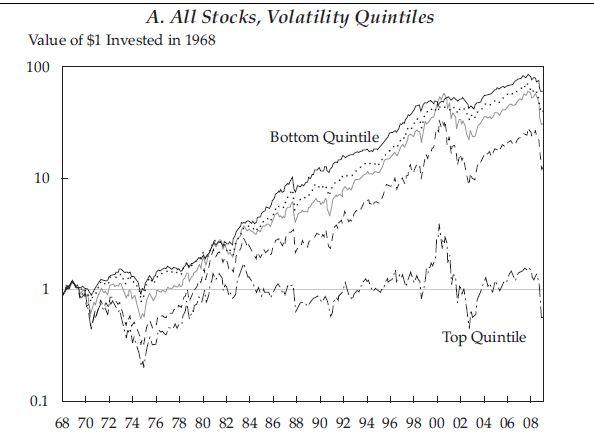
\includegraphics[height=0.52\textheight,keepaspectratio]{figures/slide38_img.jpg}
\end{figure}
\begin{center}\small Source: my calculation based on Kenneth French's data.\end{center}
\end{column}
\begin{column}{0.50\textwidth}
\textbf{Explanation: investors' preference for lottery-type stocks}
\begin{itemize}
  \item Investors accept bets with a small chance of winning big but a lower average return: people prefer a 1/1000 chance of winning \$5,000 over \$10 with certainty (Tversky and Kahneman, 1992)
  \item High-volatility stocks resemble a lottery --- and are thus \emph{overvalued}
  \item Evidence: Kumar (2009) --- retail investors who spend more on lotteries also buy more high-volatility stocks
\end{itemize}
\end{column}
\end{columns}
\note{Note that risk-averse investors would reject the fair game.}
\end{frame}

% [src: 40, 41, 42]
\begin{frame}{Profitability, Investment, and Share Issuance}
\begin{description}
  \item[Profitability / quality] More profitable firms (quintile 5) earn \emph{higher} returns than less profitable firms (quintile 1). Profitability is part of a broad set of quality characteristics (Asness, Frazzini, Pedersen 2018: profitability, profit growth, low earnings volatility, low credit risk, high dividend yield) --- despite being \emph{less} risky, quality stocks earn higher returns
  \item[Investment] Firms that invest more (quintile 5) earn \emph{lower} average returns than firms that invest less --- markets may be too optimistic about high-investment firms, pushing up prices and lowering returns
  \item[Share issuance] Issuers (top 20\%) underperform repurchasers (issuance $<0$) --- consistent with \emph{market timing}: managers issue when they believe their stock is overvalued, repurchase when undervalued
\end{description}
\vspace{0.2em}
\begin{center}
\small Source (all three): my calculation based on Kenneth French's data.
\end{center}
% TODO: recreate charts (native PowerPoint charts on source slides 40, 41, 42 — no images recovered).
\end{frame}

% [src: 43, 44]
\begin{frame}{Interpreting Anomalies}
Is a higher return sufficient evidence of an anomaly? \textbf{No} --- we need positive \emph{alpha} (risk-adjusted return), which raises the question of the correct asset pricing model.
\begin{description}
  \item[1.\ Risk] Anomalies are compensation for taking risks (value and small stocks are riskier) --- but hard to justify for profitability and low volatility
  \item[2.\ Inefficient markets] Investor biases in trading lead to market inefficiency
  \item[3.\ Data mining] Search data repeatedly and you find patterns by chance; some anomalies cannot be replicated (Hou, Xue, and Zhang, 2018). Real anomalies should exist across different markets/assets --- value, size, and momentum may be real
\end{description}
\begin{figure}
\centering

\includegraphics[height=0.34\textheight,keepaspectratio]{figures/slide44_img.jpg}
\end{figure}
\end{frame}

% [src: 45]
\begin{frame}{Momentum Is Pervasive: International Evidence}
The momentum effect exists in the majority of countries --- especially strong in Europe, weaker among Asian countries.
\begin{figure}
\centering
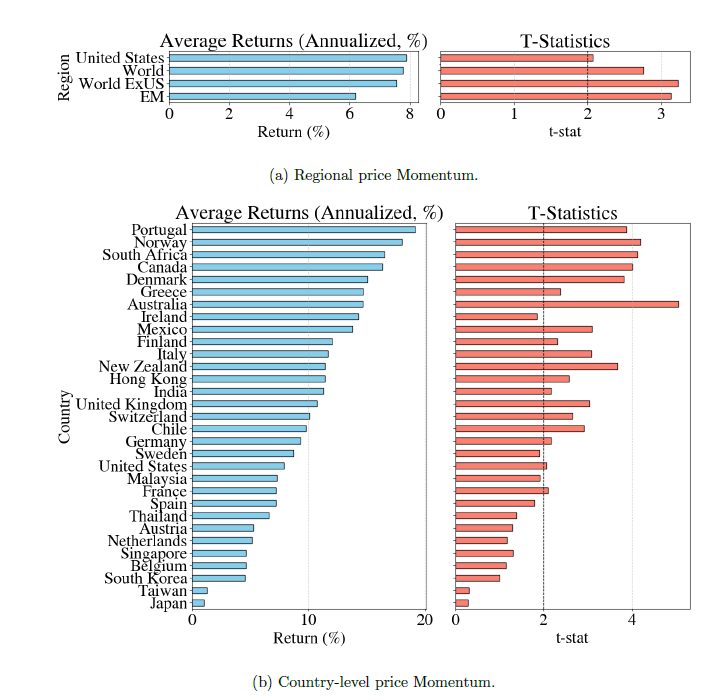
\includegraphics[height=0.60\textheight,keepaspectratio]{figures/slide45_img_flat.png}
\end{figure}
\begin{center}
\small Baltussen, Dom, Van Vliet, and Vidojevic (2025)
\end{center}
\end{frame}

% [src: 46, 47]
\begin{frame}{Anomalies May Be Real, But\ldots}
\textbf{\ldots costly to exploit due to trading costs}
\begin{itemize}
  \item Most anomalies exist only in small-cap stocks with high transaction costs and short-selling constraints
\end{itemize}
\textbf{\ldots profits may decay over time}
\begin{itemize}
  \item Improved trading technology makes markets more efficient; investors learn; more competitors trade the anomalies
\end{itemize}
\begin{columns}
\begin{column}{0.50\textwidth}
\begin{figure}
\centering

\includegraphics[width=\linewidth,keepaspectratio]{figures/slide47_img.png}
\end{figure}
\end{column}
\begin{column}{0.48\textwidth}
\begin{figure}
\centering

\includegraphics[width=\linewidth,keepaspectratio]{figures/slide47_img1.png}
\end{figure}
\end{column}
\end{columns}
\begin{center}\small Post-earnings announcement drift across periods --- Source: Martineau (2021)\end{center}
\note{Post-earnings announcement drift no longer exists in the 2011--2015 period.}
\end{frame}

% [src: 48]
\begin{frame}{The Paradox of Efficiency}
\begin{description}
  \item[Grossman--Stiglitz paradox] If everyone believes markets are efficient, no one will bother to seek information --- making prices inefficient. \emph{The very act of trying to beat the market is what makes it efficient.}
\end{description}
\vspace{0.3em}
\textbf{The EMH as a lens:}
\begin{itemize}
  \item It is the default null hypothesis; the burden of proof is on the active manager
  \item Remarkably robust, but not a perfect description of reality
  \item Finance has evolved from ``are markets efficient?'' to \emph{how} efficient, under what conditions, and where the persistent inefficiencies are
\end{itemize}
\end{frame}

% ============ SMART BETA ============

% [src: 49]
\section{Smart Beta ETFs}

% [src: 50]
\begin{frame}{Smart Beta ETFs}
All these anomalies sound great --- but can investors benefit from them?
\begin{itemize}
  \item In the past: no easy way --- only high-net-worth investors could access hedge funds investing systematically in these strategies
  \item Recently: many \textbf{Smart Beta ETFs} allow retail investors to invest in such strategies easily
\end{itemize}
\vspace{0.3em}
\begin{description}
  \item[Smart Beta ETF] An exchange-traded fund tracking a \emph{non-market-cap-weighted} index, constructed on transparent, rules-based criteria that tilt portfolio exposures toward one or more investment factors --- proven hedge-fund strategies at much lower cost and with great transparency
\end{description}
\end{frame}

% [src: 51]
\begin{frame}{Smart Beta ETFs: Passive or Active?}
Smart beta \emph{blurs the line}: \textbf{passive} because it is rules-based, transparent, and low cost relative to active funds; \textbf{active} because it makes deliberate choices about index design --- which factors to target, how to measure them, how to weight securities, how often to rebalance.
\begin{table}
\centering
\small
\begin{tabular}{llll}
\toprule
\textbf{Strategy} & \textbf{Approach} & \textbf{Avg.\ expense ratio} & \textbf{Factor transparency} \\
\midrule
Market-cap ETF & Full passive replication & $\sim$0.16\% & None \\
Smart Beta ETF & Rules-based factor tilt & $\sim$0.33\% & High \\
Active Quant Fund & Model-driven, PM discretion & $\sim$0.60\% & Moderate \\
Traditional Active & Stock-picker judgment & $\sim$0.62\% & Low \\
\bottomrule
\end{tabular}
\end{table}
\vspace{-0.2em}
\begin{center}
\footnotesize Asset-weighted averages, Morningstar 2025 Fund Fee Study (2024 data); smart-beta figure is an issuer-reported average. Cheapest S\&P 500 ETFs: SPLG 0.02\%, VOO/IVV 0.03\%.
\end{center}
\end{frame}

% [src: 52]
\begin{frame}{The Academic Genesis --- Factor Investing}
\begin{itemize}
  \item \textbf{CAPM}: only one systematic risk factor --- market beta --- prices securities in equilibrium
  \item \textbf{Fama and French (1993)}: two additional factors --- size (SMB: small minus big) and value (HML: high minus low book-to-market) --- explain a large portion of the cross-section of equity returns that CAPM cannot
  \item \textbf{Carhart (1997)}: added momentum (MOM: past-12-month winners minus losers, skipping one month) --- the canonical four-factor model
  \item \textbf{Fama and French (2015)}: extended with two factors related to investment and profitability
\end{itemize}
\begin{figure}
\centering

\includegraphics[height=0.35\textheight,keepaspectratio]{figures/slide52_img_flat.png}
\end{figure}
\end{frame}

% [src: 53]
\begin{frame}{The Six Core Investable Factors}
Despite the proliferation of proposed factors, practitioner consensus --- reflected in products from BlackRock iShares, MSCI, and S\&P DJI --- has converged on a manageable set:
\begin{table}
\centering
\footnotesize
\begin{tabular}{lp{0.26\textwidth}p{0.22\textwidth}p{0.22\textwidth}}
\toprule
\textbf{Factor} & \textbf{Definition} & \textbf{Measurement} & \textbf{Economic rationale} \\
\midrule
Value & Cheap vs.\ expensive stocks & P/B, P/E, P/S ratios & Risk compensation or mean-reversion of mispricing \\
Size & Small-cap vs.\ large-cap & Market capitalization & Liquidity/information risk premium \\
Momentum & Past winners vs.\ losers & 12--1 month returns & Underreaction, behavioral extrapolation \\
Quality & High profitability, stable earnings & ROE, accruals, leverage & Distress risk; earnings persistence \\
Low Volatility & Low-risk stocks & Historical return variance & Lottery demand, leverage constraints \\
Investment & Conservative vs.\ aggressive capex & Asset growth, capex & Asset pricing / q-theory \\
\bottomrule
\end{tabular}
\end{table}
\end{frame}

% [src: 54]
\begin{frame}{The Six Core Investable Factors}
\begin{figure}
\centering
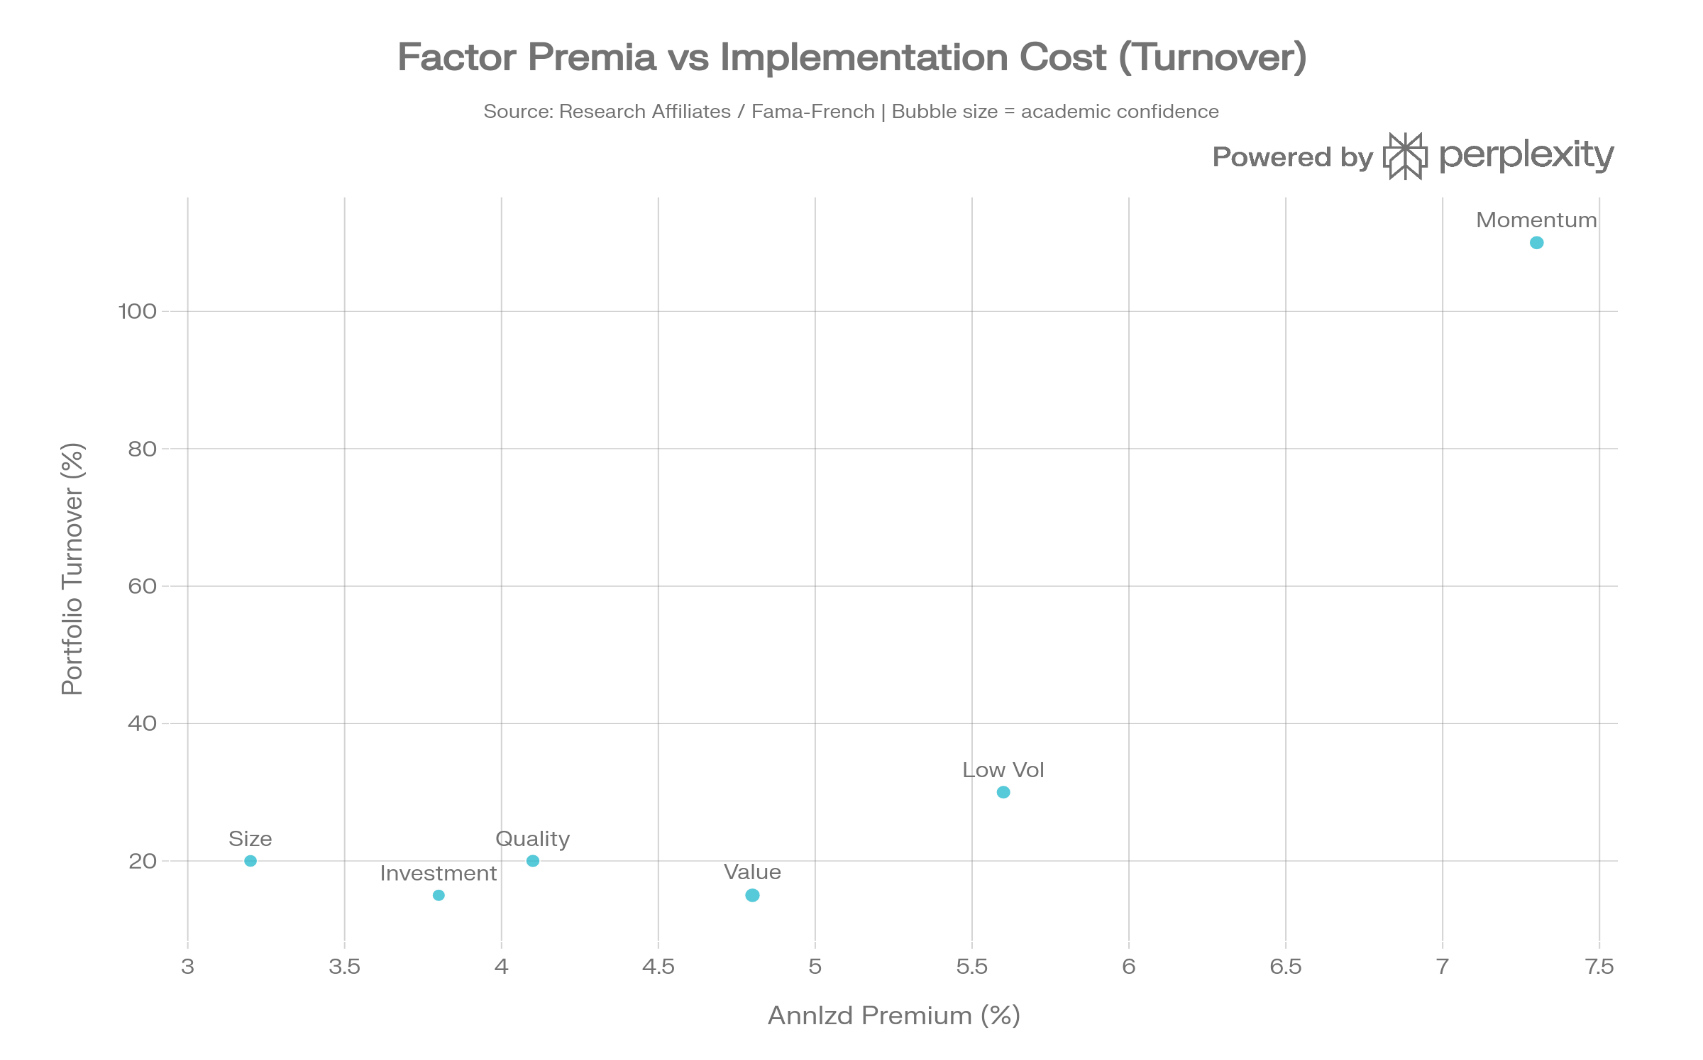
\includegraphics[height=0.68\textheight,keepaspectratio]{figures/slide54_img_flat.png}
\end{figure}
\end{frame}

% [src: 55]
\begin{frame}{Factor Cyclicality}
Factor premia are \emph{not constant} --- they vary systematically with the macroeconomic and credit cycle:
\begin{itemize}
  \item \textbf{Expansions} (rising growth): Value and Momentum perform best; Low Volatility lags
  \item \textbf{Contractions} (falling growth): Quality and Low Volatility provide defensive outperformance; Value and Momentum suffer sharply
  \item \textbf{Recoveries}: Size (equal weight) and Value tend to outperform as risk appetite returns
\end{itemize}
\begin{figure}
\centering
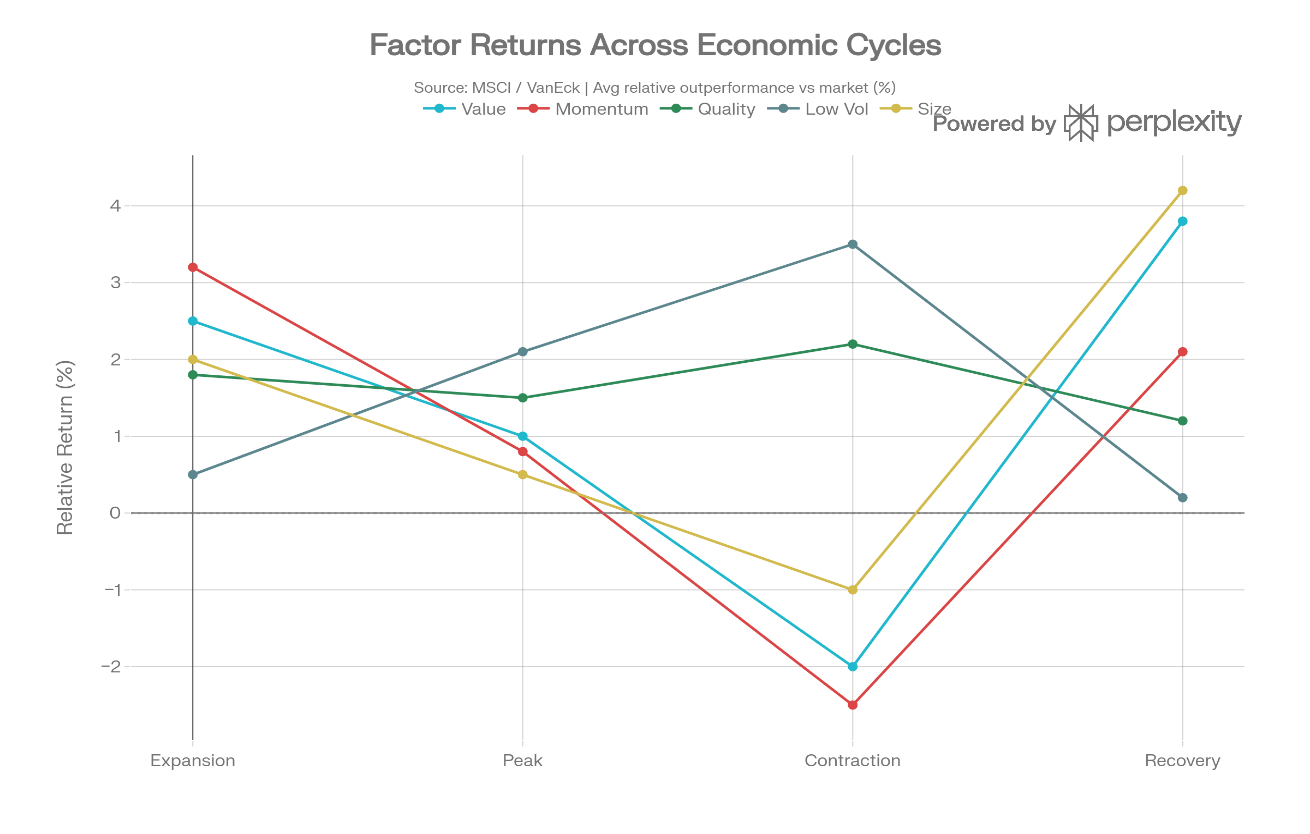
\includegraphics[height=0.44\textheight,keepaspectratio]{figures/slide55_img_flat.png}
\end{figure}
\end{frame}

% [src: 56]
\begin{frame}{Multi-Factor Diversification}
Factors exhibit \textbf{low to negative correlations} with each other in excess-return space. Combining them substantially reduces tracking error without proportionately reducing expected returns.
\begin{figure}
\centering
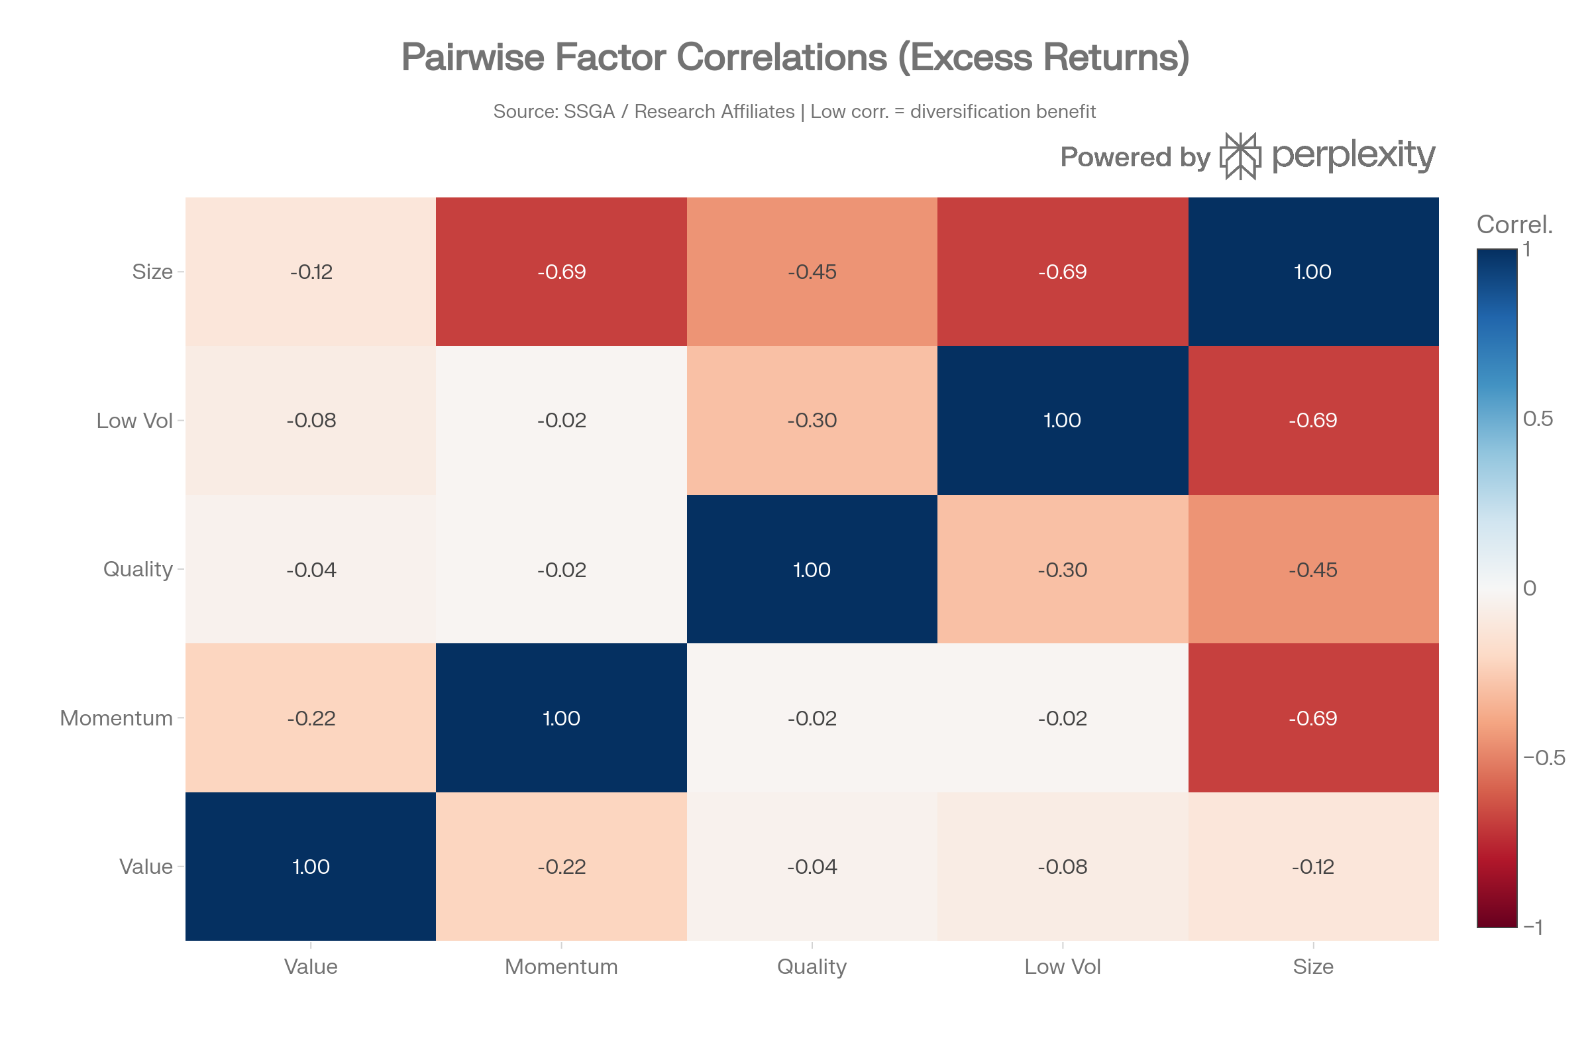
\includegraphics[height=0.62\textheight,width=0.94\textwidth,keepaspectratio]{figures/slide56_img_flat.png}
\end{figure}
\end{frame}

% [src: 57]
\begin{frame}{A ``Quality'' Smart Beta ETF}
\begin{columns}
\begin{column}{0.60\textwidth}
\begin{figure}
\centering

\includegraphics[height=0.44\textheight,keepaspectratio]{figures/slide57_img.png}
\end{figure}
\end{column}
\begin{column}{0.36\textwidth}
\begin{figure}
\centering
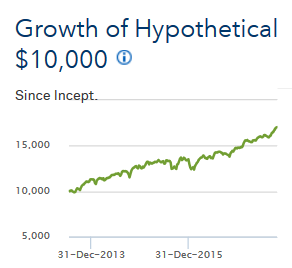
\includegraphics[height=0.40\textheight,keepaspectratio]{figures/slide57_img1.png}
\end{figure}
\end{column}
\end{columns}
\note{The expense ratio for smart beta ETFs is usually much lower than the cost of investing in hedge funds employing the same strategies.}
\end{frame}

% [src: 58]
\begin{frame}{A ``Momentum'' Smart Beta ETF}
\begin{figure}
\centering

\includegraphics[height=0.66\textheight,keepaspectratio]{figures/slide58_img_flat.png}
\end{figure}
\end{frame}

% [src: 59]
\begin{frame}{Performance Evidence --- Theory vs.\ Reality}
Factor returns look strong in academic backtests but shrink markedly once strategies become investable:
\begin{itemize}
  \item \textbf{McLean and Pontiff (\emph{Journal of Finance}, 2016):} across 97 published anomalies, returns decline by $\sim$26\% out-of-sample and by $\sim$32\% after publication
  \item \textbf{Hou, Xue, and Zhang (\emph{AER}, 2020):} under replicated tests, only 22\% of 452 studied anomalies remain significant
\end{itemize}
\begin{figure}
\centering
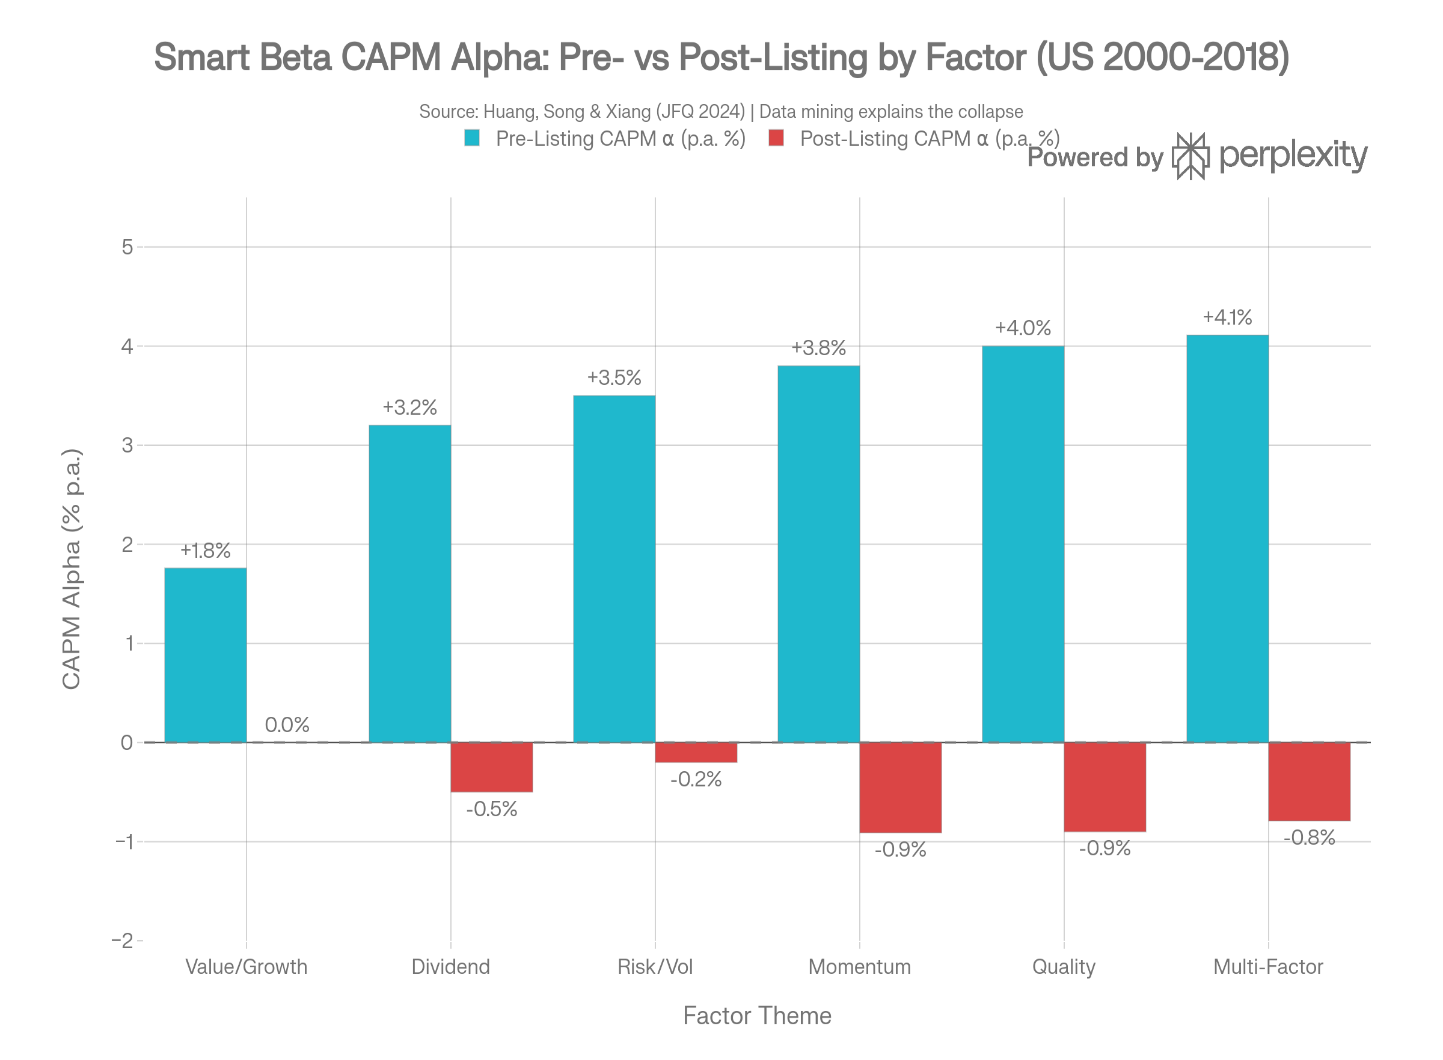
\includegraphics[height=0.44\textheight,keepaspectratio]{figures/slide59_img_flat.png}
\end{figure}
\note{Backtest-vs-live performance decay: figure from the smart-beta ETF listing literature --- original citation pending verification by the instructor (flagged 2026-09-09); the deck's earlier ``$+2.77\%$/yr pre-listing, $-3.22\%$/yr post-listing'' figures did not match McLean--Pontiff and were replaced.}
\end{frame}

% [src: 60]
\begin{frame}{Industry Trends}
Smart beta AUM grew from \$160 billion in 2008 to approximately \$2.6 trillion by early 2026 (Morningstar) --- a more than sixteenfold increase since 2008.
\begin{columns}
\begin{column}{0.54\textwidth}
\begin{figure}
\centering
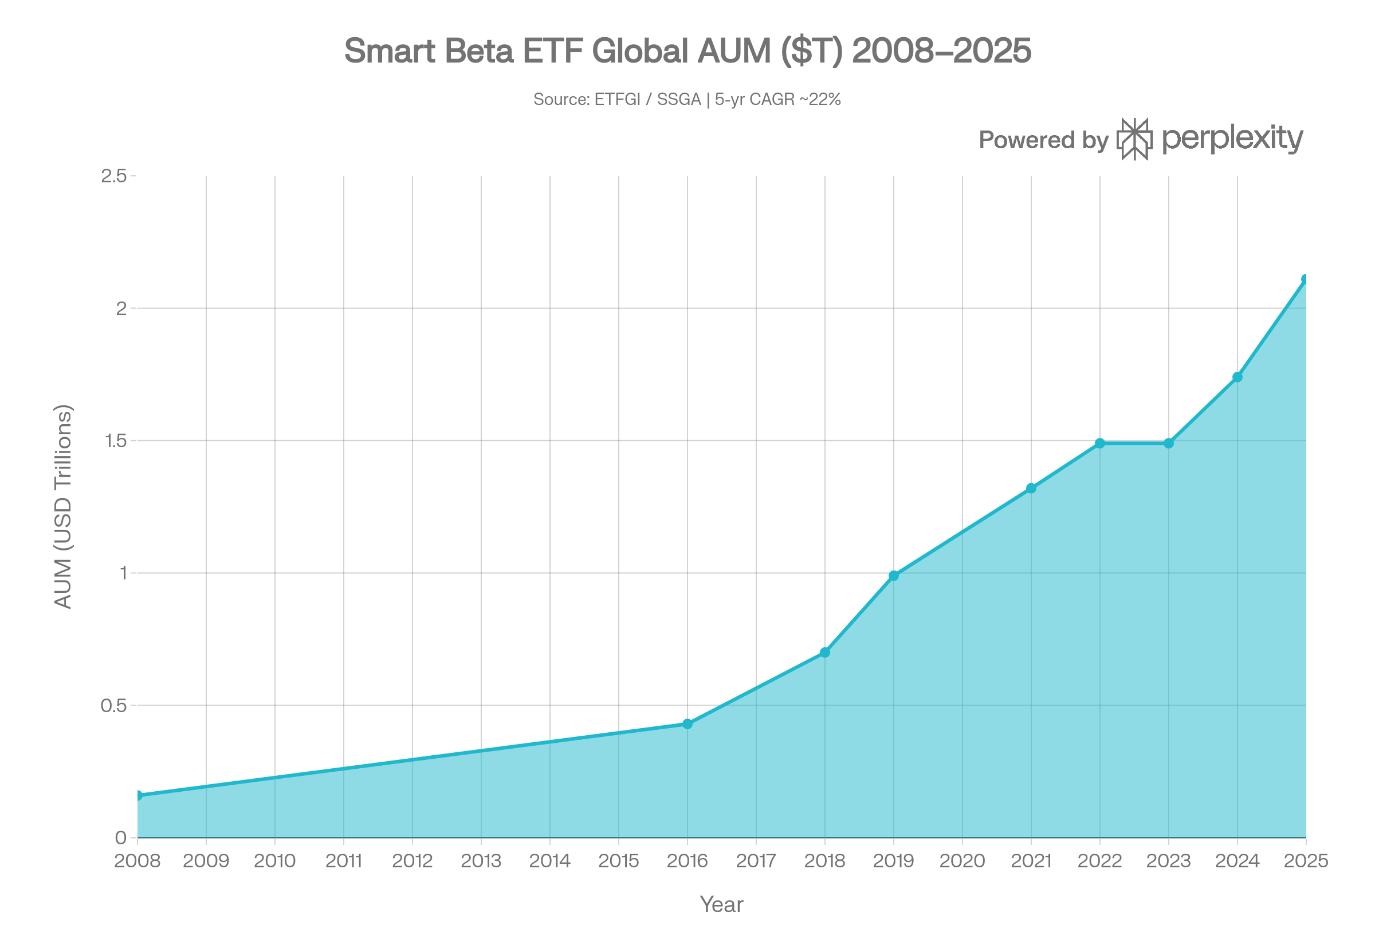
\includegraphics[height=0.46\textheight,keepaspectratio]{figures/slide60_img_flat.png}
\end{figure}
\end{column}
\begin{column}{0.42\textwidth}
\begin{figure}
\centering
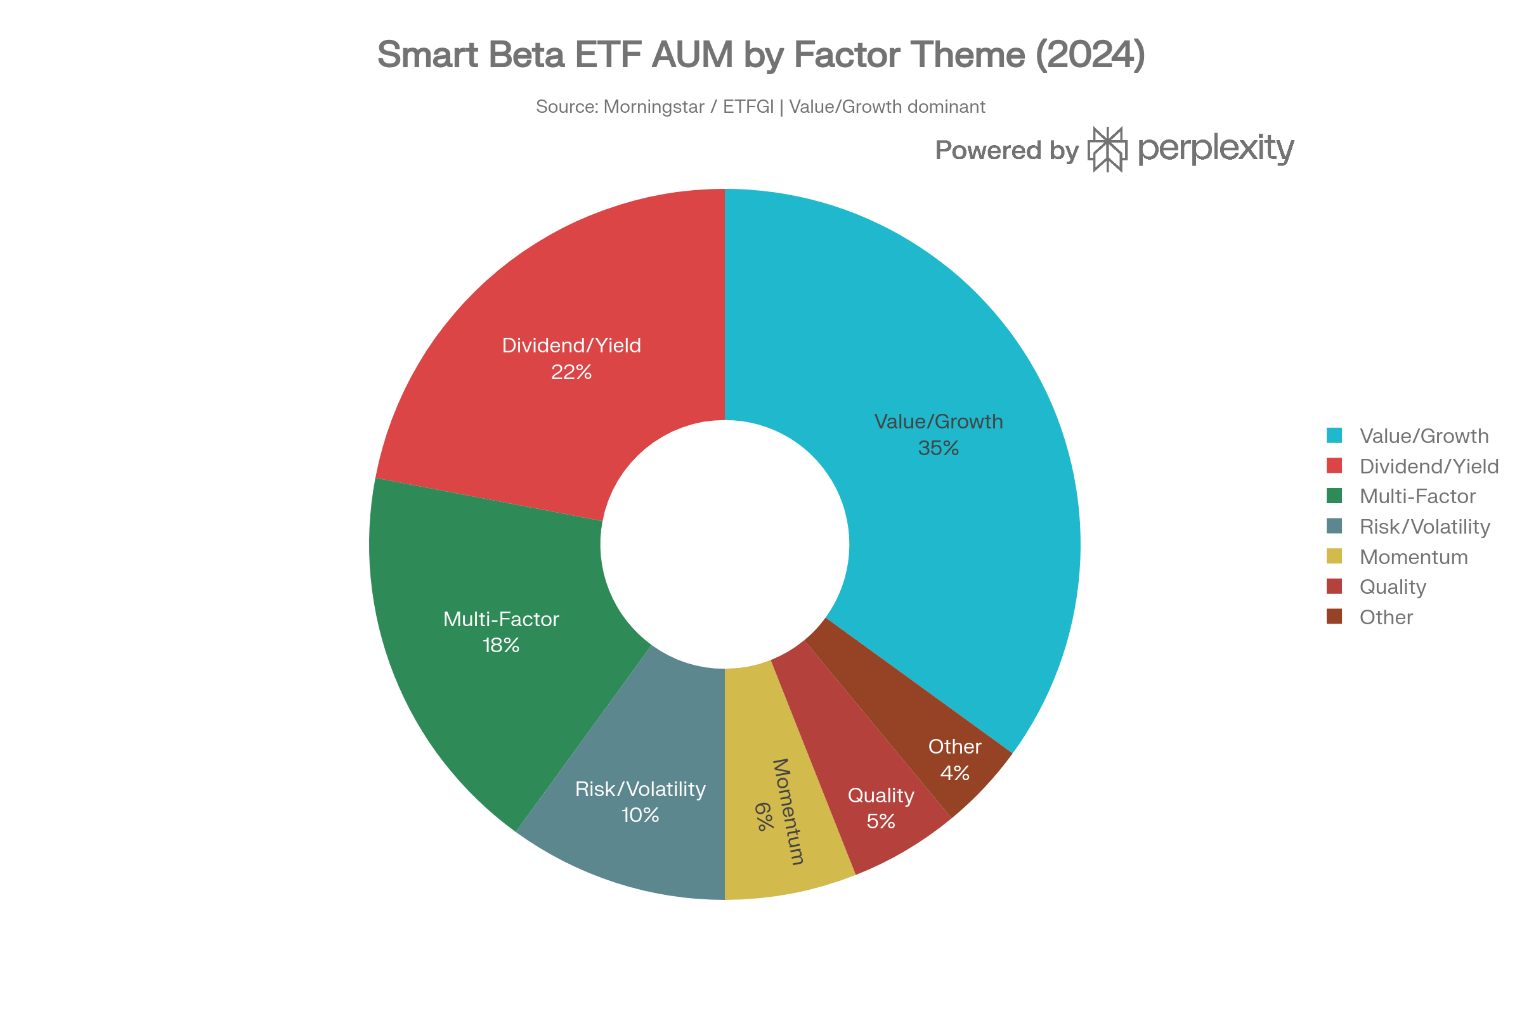
\includegraphics[height=0.40\textheight,keepaspectratio]{figures/slide60_img1_flat.png}
\end{figure}
\end{column}
\end{columns}
\note{By factor theme, value/growth and dividend ETFs dominate AUM, reflecting their longer history and broader retail appeal. Multi-factor and momentum strategies are growing fastest in product launches, though their performance record is most challenged.}
\end{frame}

% [src: 61, 62]
\begin{frame}{Portfolio Construction Applications}
\textbf{Core--satellite framework} --- the most common deployment:
\begin{itemize}
  \item Passive market-cap \emph{core} (60--80\% of equity allocation): low-cost broad-market exposure
  \item Smart beta \emph{satellites} (20--40\%): factor tilts toward desired outcomes --- higher expected return, lower volatility, or income
\end{itemize}
\vspace{0.3em}
\textbf{Strategic factor allocation:}
\begin{itemize}
  \item Long-horizon investors (pensions, endowments): value, size, profitability --- longest academic documentation, strongest risk-based rationale
  \item Volatility-sensitive investors: min-volatility and quality reduce downside capture
  \item Income-focused investors: high-dividend-yield ETFs (value tilt plus current income)
\end{itemize}
\vspace{0.3em}
\textbf{Factor timing --- mostly inadvisable:} the empirical literature on factor timing is discouraging; rotating on relative factor valuations has not produced consistently strong out-of-sample results. Consensus: maintain diversified, rebalanced multi-factor exposures.
\end{frame}

% ============ SUMMARY ============

% [src: 63, 64]
\begin{frame}{Key Takeaways}
\begin{description}
  \item[EMH] Security prices fully reflect all available information; new information is random $\Rightarrow$ prices follow a random walk and are unpredictable
  \item[Three forms] Weak (past prices/volume --- technical analysis useless); semi-strong (all public info --- fundamental analysis useless); strong (all info --- no one beats the market, including insiders)
  \item[Evidence against] Momentum (violates weak form); post-earnings drift (violates semi-strong); asset bubbles (dot-com); size, value, low volatility, profitability, and investment effects
  \item[Interpreting anomalies] Risk compensation; behavioral biases (overreaction, lottery preference); data mining (non-replicable patterns)
  \item[Practical implications] Smart beta ETFs let retail investors systematically exploit anomalies via rules-based, transparent strategies; the Grossman--Stiglitz paradox --- trying to beat the market is what makes it efficient
\end{description}
\end{frame}

\end{document}
